\documentclass{article}
% Adjust the relative path to point to the latex-templates directory from:
% content/resources/study-materials/32-ict/sem-4/4343204-embedded-systems/

% content/resources/templates/preamble.tex
\usepackage[margin=0.6in]{geometry}
\author{Milav Dabgar}
\usepackage{amsmath,amssymb,amsthm}
\usepackage{booktabs}
\usepackage{multirow}
\usepackage{xcolor}
\usepackage{tcolorbox}
\tcbuselibrary{breakable,skins}
\usepackage[colorlinks=true,linkcolor=blue]{hyperref}
\usepackage{titlesec}
\usepackage{enumitem}
\usepackage{tikz}
\usepackage{pgfplots}
\usepackage{circuitikz}
\usepackage[version=4]{mhchem}
\usepackage{longtable}
\usepackage{array}
\usepackage{float}
\usepackage{caption}
\usepackage{listings}

\lstset{
  basicstyle=\small\ttfamily,
  breaklines=true,
  breakatwhitespace=false,
  postbreak=\mbox{\textcolor{red}{$\hookrightarrow$}\space},
  float=false,
  numbers=left,
  numberstyle=\tiny\color{gray},
  numbersep=10pt,
  xleftmargin=2em,
  keywordstyle=\color{blue},
  commentstyle=\color{green!60!black},
  stringstyle=\color{purple},
  backgroundcolor=\color{gray!5},
  showstringspaces=false,
  tabsize=2,
  captionpos=b,
  keepspaces=true,
  columns=flexible
}

\pgfplotsset{compat=1.18}
\usetikzlibrary{shapes,arrows,positioning,calc,patterns,decorations.pathmorphing,decorations.markings,arrows.meta}

% Color scheme
\definecolor{headcolor}{RGB}{0,102,204}
\definecolor{keycolor}{RGB}{220,20,60}
\definecolor{solutioncolor}{RGB}{34,139,34}
\definecolor{mnemoniccolor}{RGB}{148,0,211}
\definecolor{codecolor}{RGB}{0,0,100}

% Spacing
\setlength{\parskip}{3pt}
\setlist[itemize]{nosep}
\setlist[enumerate]{nosep}

% Title formatting
\titleformat{\section}{\Large\bfseries\color{headcolor}}{\thesection}{1em}{}
\titleformat{\subsection}{\large\bfseries\color{headcolor}}{\thesubsection}{1em}{}

% Pandoc tightlist compatibility
\providecommand{\tightlist}{%
  \setlength{\itemsep}{0pt}\setlength{\parskip}{0pt}}

% Pandoc longtable compatibility
\newcounter{none}
\def\thenone{}


% content/resources/templates/english-boxes.tex

% Custom environments
\newtcolorbox{solutionbox}{
 breakable,
 enhanced,
 colback=solutioncolor!5!white,
 colframe=solutioncolor!75!black,
 fonttitle=\bfseries,
 title=Solution
}

\newtcolorbox{solutionboxnobreak}{
 colback=solutioncolor!5!white,
 colframe=solutioncolor!75!black,
 fonttitle=\bfseries,
 title=Solution
}

\newtcolorbox{keyformula}{
 breakable,
 enhanced,
 colback=keycolor!5!white,
 colframe=keycolor!75!black,
 fonttitle=\bfseries,
 title=Key Formula
}

\newtcolorbox{mnemonicboxenv}{
 breakable,
 enhanced,
 colback=mnemoniccolor!5!white,
 colframe=mnemoniccolor!75!black,
 fonttitle=\bfseries,
 title=Mnemonic
}

\newcommand{\mnemonicbox}[1]{%
  \begin{mnemonicboxenv}
    #1
  \end{mnemonicboxenv}
}


% Custom commands for GTU solutions
% This file defines semantic commands for consistent formatting

% Question command with automatic formatting
\newcommand{\question}[2]{%
  \section*{Question #1}%
  \textbf{#2}%
}

% OR question variant
\newcommand{\questionor}[2]{%
  \section*{Question #1 OR}%
  \textbf{#2}%
}

% Proper table environment with caption
\newenvironment{answertable}[1]{%
  \begin{table}[htbp]
  \centering
  \caption{#1}
}{%
  \end{table}
}

% Proper figure environment for diagrams
\newenvironment{answerdiagram}[1]{%
  \begin{figure}[htbp]
  \centering
  \caption{#1}
}{%
  \end{figure}
}

% Semantic markup for key terms
\newcommand{\keyword}[1]{\textbf{#1}}
\newcommand{\code}[1]{\texttt{#1}}
\newcommand{\classname}[1]{\texttt{#1}}
\newcommand{\methodname}[1]{\texttt{#1}}

% Proper quotation marks
\newcommand{\mnemonic}[1]{``#1''}


\title{Embedded System (4343204) -- Summer 2024 Solution}
\date{June 21, 2024}

\begin{document}
\maketitle

\questionmarks{1(a)}{3}{Draw AVR status register.}

\begin{solutionbox}
The AVR Status Register (SREG) contains information about the result of arithmetic operations and controls interrupts.

\textbf{Diagram:}

\begin{center}
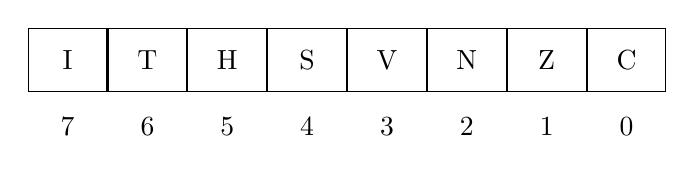
\begin{tikzpicture}[node distance=0cm]
    \node [draw, minimum width=1cm, minimum height=0.8cm] (I) {I};
    \node [draw, minimum width=1cm, minimum height=0.8cm, right=0cm of I] (T) {T};
    \node [draw, minimum width=1cm, minimum height=0.8cm, right=0cm of T] (H) {H};
    \node [draw, minimum width=1cm, minimum height=0.8cm, right=0cm of H] (S) {S};
    \node [draw, minimum width=1cm, minimum height=0.8cm, right=0cm of S] (V) {V};
    \node [draw, minimum width=1cm, minimum height=0.8cm, right=0cm of V] (N) {N};
    \node [draw, minimum width=1cm, minimum height=0.8cm, right=0cm of N] (Z) {Z};
    \node [draw, minimum width=1cm, minimum height=0.8cm, right=0cm of Z] (C) {C};
    
    \node [below=0.2cm of I] {7};
    \node [below=0.2cm of T] {6};
    \node [below=0.2cm of H] {5};
    \node [below=0.2cm of S] {4};
    \node [below=0.2cm of V] {3};
    \node [below=0.2cm of N] {2};
    \node [below=0.2cm of Z] {1};
    \node [below=0.2cm of C] {0};
\end{tikzpicture}
\end{center}

\begin{itemize}
    \item \keyword{I (bit 7)}: Global Interrupt Enable
    \item \keyword{T (bit 6)}: Bit Copy Storage
    \item \keyword{H (bit 5)}: Half Carry Flag
    \item \keyword{S (bit 4)}: Sign Flag (S = N$\oplus$V)
    \item \keyword{V (bit 3)}: Two's Complement Overflow
    \item \keyword{N (bit 2)}: Negative Flag
    \item \keyword{Z (bit 1)}: Zero Flag
    \item \keyword{C (bit 0)}: Carry Flag
\end{itemize}
\end{solutionbox}

\begin{mnemonicbox}
\mnemonic{I Take Health Seriously, Very Nice Zero Carry}
\end{mnemonicbox}

\questionmarks{1(b)}{4}{Explain Harvard Architecture in the AVR.}

\begin{solutionbox}
Harvard Architecture in AVR separates program and data memory, allowing simultaneous access to both.

\textbf{Diagram:}

\begin{center}
\begin{tikzpicture}[node distance=2cm, auto]
    \node [gtu block] (CPU) {CPU};
    \node [gtu block, above right=1cm and 2cm of CPU] (PM) {Program Memory};
    \node [gtu block, below right=1cm and 2cm of CPU] (DM) {Data Memory};
    
    \path [gtu arrow] (CPU) -- node {Instruction Bus} (PM);
    \path [gtu arrow] (CPU) -- node {Data Bus} (DM);
\end{tikzpicture}
\end{center}

\begin{itemize}
    \item \keyword{Program Memory}: Stores instructions in Flash memory
    \item \keyword{Data Memory}: Contains SRAM, registers, and I/O registers
    \item \keyword{Separate Buses}: Different buses for program and data
    \item \keyword{Parallel Access}: Can fetch instruction and access data simultaneously
\end{itemize}
\end{solutionbox}

\begin{mnemonicbox}
\mnemonic{Separate Places for Data And Programs}
\end{mnemonicbox}

\questionmarks{1(c)}{7}{Discuss real time operating system.}

\begin{solutionbox}
Real-Time Operating System (RTOS) manages tasks with strict timing requirements, ensuring predictable response times.

\begin{center}
\captionof{table}{Key Features of RTOS}
\begin{tabulary}{\linewidth}{|L|L|}
\hline
\textbf{Feature} & \textbf{Description} \\ \hline
Task Scheduling & Prioritizes tasks based on urgency \\ \hline
Deterministic & Guaranteed response times for events \\ \hline
Preemptive & Critical tasks can interrupt lower priority ones \\ \hline
Memory Management & Efficient memory allocation without fragmentation \\ \hline
Low Latency & Minimal delay between event and response \\ \hline
Multitasking & Handles multiple tasks concurrently \\ \hline
\end{tabulary}
\end{center}

\begin{itemize}
    \item \keyword{Task-based}: Divides program into independent tasks
    \item \keyword{Interrupt Handling}: Fast response to external events
    \item \keyword{Synchronization}: Provides semaphores and mutexes for task coordination
    \item \keyword{Resource Management}: Prevents resource conflicts
    \item \keyword{Small Footprint}: Optimized for limited hardware resources
\end{itemize}
\end{solutionbox}

\begin{mnemonicbox}
\mnemonic{Tasks Run On Strict Timelines}
\end{mnemonicbox}

\questionmarks{1(c OR)}{7}{Discuss criteria for choosing microcontroller for embedded system.}

\begin{solutionbox}
Selecting the right microcontroller requires evaluating several key factors to match application requirements.

\begin{center}
\captionof{table}{Microcontroller Selection Criteria}
\begin{tabulary}{\linewidth}{|L|L|}
\hline
\textbf{Criterion} & \textbf{Considerations} \\ \hline
Processing Power & CPU speed, bit width (8/16/32-bit) \\ \hline
Memory & Flash, RAM, EEPROM sizes \\ \hline
Power Consumption & Sleep modes, operating voltage \\ \hline
I/O Capabilities & Number of ports, special functions \\ \hline
Peripherals & Timers, ADC, communication interfaces \\ \hline
Cost & Unit price, development tools cost \\ \hline
Development Support & Tools, documentation, community \\ \hline
\end{tabulary}
\end{center}

\begin{itemize}
    \item \keyword{Application Needs}: Match controller to task complexity
    \item \keyword{Real-time Requirements}: Response time constraints
    \item \keyword{Environmental Factors}: Temperature, noise, vibration
    \item \keyword{Form Factor}: Physical size and packaging
    \item \keyword{Future Expansion}: Room for feature growth
\end{itemize}
\end{solutionbox}

\begin{mnemonicbox}
\mnemonic{Power, Memory, I/O, Peripherals, Cost}
\end{mnemonicbox}

\questionmarks{2(a)}{3}{Define embedded system and draw its general block diagram.}

\begin{solutionbox}
An embedded system is a dedicated computer system designed for specific functions within a larger mechanical or electrical system.

\textbf{Diagram:}

\begin{center}
\begin{tikzpicture}[node distance=2.5cm, auto]
    \node [gtu block] (input) {Input\\Devices};
    \node [gtu block, right=of input] (proc) {Processing\\Unit};
    \node [gtu block, right=of proc] (output) {Output\\Devices};
    
    \node [gtu block, below=1.5cm of input] (sensors) {Sensors};
    \node [gtu block, below=1.5cm of proc] (memory) {Memory};
    \node [gtu block, below=1.5cm of output] (actuators) {Actuators};
    
    \node [gtu block, below=1.5cm of memory] (power) {Power\\Supply};
    
    \path [gtu arrow] (input) -- (proc);
    \path [gtu arrow] (proc) -- (output);
    \path [gtu arrow, <->] (sensors) -- (input);
    \path [gtu arrow, <->] (memory) -- (proc);
    \path [gtu arrow, <->] (actuators) -- (output);
    \path [gtu arrow] (power) -- (memory);
\end{tikzpicture}
\end{center}

\begin{itemize}
    \item \keyword{Processing Unit}: Microcontroller/microprocessor
    \item \keyword{Memory}: Stores program and data
    \item \keyword{Input/Output}: Interfaces with external world
\end{itemize}
\end{solutionbox}

\begin{mnemonicbox}
\mnemonic{Processing Memory I/O Power}
\end{mnemonicbox}

\questionmarks{2(b)}{4}{List I/O registers associated with each port.}

\begin{solutionbox}
AVR microcontrollers have three primary registers for controlling each I/O port.

\begin{center}
\captionof{table}{I/O Port Registers}
\begin{tabulary}{\linewidth}{|L|L|L|}
\hline
\textbf{Register} & \textbf{Function} & \textbf{Description} \\ \hline
PORTx & Data Register & Sets output values or pull-ups \\ \hline
DDRx & Data Direction Register & Sets pin direction (1=output, 0=input) \\ \hline
PINx & Port Input Pins & Reads actual pin status \\ \hline
\end{tabulary}
\end{center}

\begin{itemize}
    \item \keyword{x represents}: A, B, C, D (port letter)
    \item \keyword{Additional Special}: Some ports have PCMSK (Pin Change Mask) registers
\end{itemize}
\end{solutionbox}

\begin{mnemonicbox}
\mnemonic{Direction, Data, Pin reading}
\end{mnemonicbox}

\questionmarks{2(c)}{7}{Explain clock and reset circuit for AVR.}

\begin{solutionbox}
The clock and reset circuits ensure proper initialization and timing of AVR operations.

\textbf{Clock Circuit Diagram:}

\begin{center}
\begin{tikzpicture}[node distance=2cm]
    \node [gtu block] (avr) {AVR};
    \node [draw, circle, left=1.5cm of avr, minimum size=0.8cm] (xtal1) {XTAL1};
    \node [draw, circle, right=1.5cm of avr, minimum size=0.8cm] (xtal2) {XTAL2};
    \node [gtu block, below=2cm of avr] (crystal) {Crystal\\Oscillator};
    \node [draw, below=0.5cm of crystal] (gnd) {GND};
    
    \path [gtu arrow] (xtal1) -- (avr);
    \path [gtu arrow] (avr) -- (xtal2);
    \path [gtu arrow] (crystal) -- (xtal1);
    \path [gtu arrow] (crystal) -- (xtal2);
    \path [gtu arrow] (crystal) -- (gnd);
\end{tikzpicture}
\end{center}

\textbf{Reset Circuit:}

\begin{center}
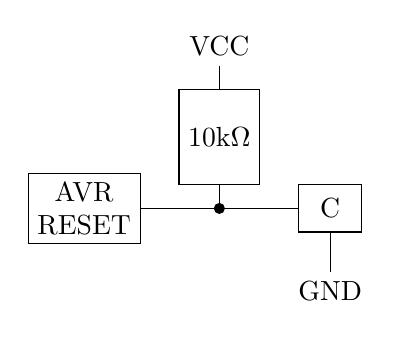
\begin{tikzpicture}[node distance=1cm]
    % VCC at top
    \node (vcc) {VCC};
    
    % 10k resistor below VCC
    \node [draw, rectangle, minimum width=0.8cm, minimum height=1.2cm, below=0.3cm of vcc] (res) {10k$\Omega$};
    
    % Junction point
    \coordinate [below=0.3cm of res] (junction);
    
    % AVR RESET to the left
    \node [draw, rectangle, minimum width=1.2cm, minimum height=0.6cm, left=1cm of junction, align=center] (avr) {AVR\\RESET};
    
    % Capacitor C to the right
    \node [draw, rectangle, minimum width=0.8cm, minimum height=0.6cm, right=1cm of junction] (cap) {C};
    
    % GND below capacitor
    \node [below=0.5cm of cap] (gnd) {GND};
    
    % Connections
    \draw (vcc) -- (res);
    \draw (res) -- (junction);
    \draw (junction) -- (avr);
    \draw (junction) -- (cap);
    \draw (cap) -- (gnd);
    
    % Add a dot at junction
    \fill (junction) circle (2pt);
\end{tikzpicture}
\end{center}

\begin{itemize}
    \item \keyword{Clock Source}: External crystal, RC oscillator, or internal oscillator
    \item \keyword{Crystal}: Provides accurate timing (1-16 MHz)
    \item \keyword{Reset Pin}: Active-low input for system restart
    \item \keyword{Power-on Reset}: Automatic reset when power applied
    \item \keyword{Brown-out Detection}: Reset if voltage drops below threshold
\end{itemize}
\end{solutionbox}

\begin{mnemonicbox}
\mnemonic{Crystal Oscillates, Reset Ensures Start}
\end{mnemonicbox}

\questionmarks{2(a OR)}{3}{Write characteristics of embedded system.}

\begin{solutionbox}
Embedded systems have unique characteristics that distinguish them from general-purpose computers.

\begin{center}
\captionof{table}{Embedded System Characteristics}
\begin{tabulary}{\linewidth}{|L|L|}
\hline
\textbf{Characteristic} & \textbf{Description} \\ \hline
Single-Function & Dedicated to specific tasks \\ \hline
Real-time & Predictable response times \\ \hline
Resource Constrained & Limited memory, power, processing \\ \hline
Reliability & Must operate continuously without fail \\ \hline
Reactive & Responds to environmental changes \\ \hline
\end{tabulary}
\end{center}

\begin{itemize}
    \item \keyword{Long Life}: Often operates for years without intervention
    \item \keyword{Often Hidden}: Integrated within larger systems
\end{itemize}
\end{solutionbox}

\begin{mnemonicbox}
\mnemonic{Single, Real-time, Resource-limited, Reliable}
\end{mnemonicbox}

\questionmarks{2(b OR)}{4}{Discuss the role of DDRx in outputting and inputting data.}

\begin{solutionbox}
DDRx (Data Direction Register) configures each pin of port x as either input or output.

\begin{center}
\captionof{table}{DDRx Role in I/O Operations}
\begin{tabulary}{\linewidth}{|L|L|L|L|}
\hline
\textbf{DDRx Value} & \textbf{PORTx Value} & \textbf{Mode} & \textbf{Function} \\ \hline
0 & 0 & Input & High-impedance mode \\ \hline
0 & 1 & Input & Pull-up enabled \\ \hline
1 & 0 & Output & Output low (0V) \\ \hline
1 & 1 & Output & Output high (VCC) \\ \hline
\end{tabulary}
\end{center}

\begin{itemize}
    \item \keyword{Direction Control}: 1 = output, 0 = input
    \item \keyword{Pin-specific}: Each bit controls individual pin
    \item \keyword{Initial State}: Default is input (all 0s)
\end{itemize}
\end{solutionbox}

\begin{mnemonicbox}
\mnemonic{Direction Determines Data flow}
\end{mnemonicbox}

\questionmarks{2(c OR)}{7}{Draw and explain ATmega32 pin diagram.}

\begin{solutionbox}
ATmega32 is a popular 8-bit AVR microcontroller with 40 pins providing various functionalities.

\textbf{Diagram:}

\begin{center}
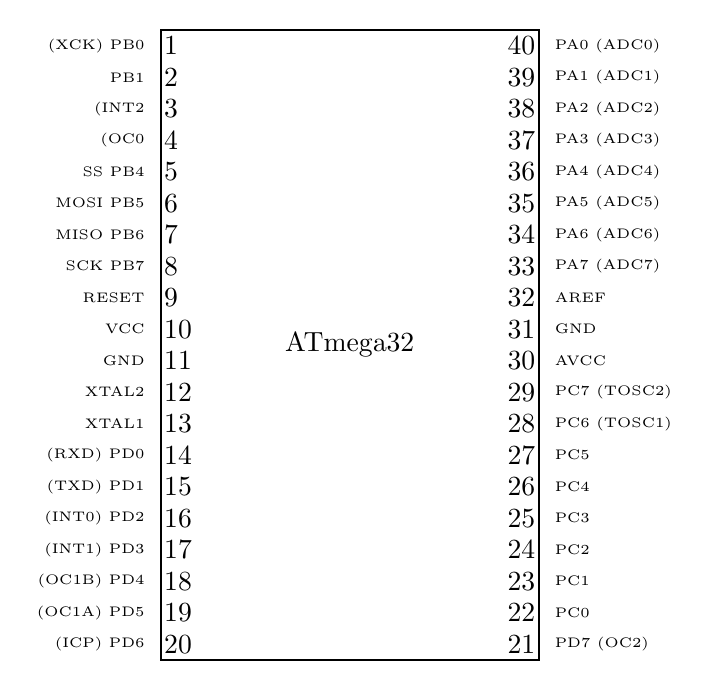
\begin{tikzpicture}[scale=0.8]
    % Draw the IC body
    \draw [thick] (0,0) rectangle (6,10);
    
    % Left side pins (1-20)
    \foreach \i/\label in {1/(XCK) PB0, 2/PB1, 3/(INT2/AIN0)PB2, 4/(OC0/AIN1)PB3, 5/SS PB4, 6/MOSI PB5, 7/MISO PB6, 8/SCK PB7, 9/RESET, 10/VCC, 11/GND, 12/XTAL2, 13/XTAL1, 14/(RXD) PD0, 15/(TXD) PD1, 16/(INT0) PD2, 17/(INT1) PD3, 18/(OC1B) PD4, 19/(OC1A) PD5, 20/(ICP) PD6} {
        \node [anchor=east, font=\tiny] at (-0.1, 10-\i*0.5+0.25) {\label};
        \node [anchor=west] at (-0.1, 10-\i*0.5+0.25) {\i};
    }
    
    % Right side pins (40-21)
    \foreach \i/\label in {40/PA0 (ADC0), 39/PA1 (ADC1), 38/PA2 (ADC2), 37/PA3 (ADC3), 36/PA4 (ADC4), 35/PA5 (ADC5), 34/PA6 (ADC6), 33/PA7 (ADC7), 32/AREF, 31/GND, 30/AVCC, 29/PC7 (TOSC2), 28/PC6 (TOSC1), 27/PC5, 26/PC4, 25/PC3, 24/PC2, 23/PC1, 22/PC0, 21/PD7 (OC2)} {
        \pgfmathsetmacro{\pos}{10-(40-\i+1)*0.5+0.25}
        \node [anchor=west, font=\tiny] at (6.1, \pos) {\label};
        \node [anchor=east] at (6.1, \pos) {\i};
    }
    
    \node at (3,5) {ATmega32};
\end{tikzpicture}
\end{center}

\begin{itemize}
    \item \keyword{Port A (PA0-PA7)}: 8-bit bidirectional port with ADC inputs
    \item \keyword{Port B (PB0-PB7)}: 8-bit port with SPI, timers, and external interrupts
    \item \keyword{Port C (PC0-PC7)}: 8-bit bidirectional port with TWI support
    \item \keyword{Port D (PD0-PD7)}: 8-bit port with USART, external interrupts, and PWM
    \item \keyword{Power/Ground}: VCC, GND, AVCC, AREF
    \item \keyword{Clock}: XTAL1/XTAL2 for external oscillator
    \item \keyword{Reset}: Active-low reset input
\end{itemize}
\end{solutionbox}

\begin{mnemonicbox}
\mnemonic{ABCD Ports Around Power Clock Reset}
\end{mnemonicbox}

\questionmarks{3(a)}{3}{Explain Program Counter (PC) register for ATmega32.}

\begin{solutionbox}
Program Counter (PC) is a 16-bit register that tracks the address of the next instruction to execute.

\textbf{Diagram:}

\begin{center}
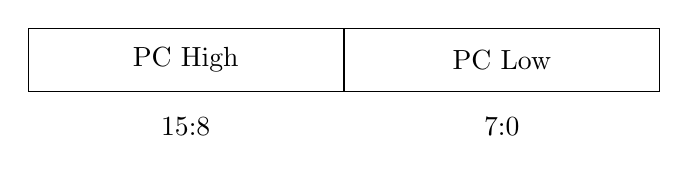
\begin{tikzpicture}[node distance=0cm]
    \node [draw, minimum width=4cm, minimum height=0.8cm] (pch) {PC High};
    \node [draw, minimum width=4cm, minimum height=0.8cm, right=0cm of pch] (pcl) {PC Low};
    
    \node [below=0.2cm of pch] {15:8};
    \node [below=0.2cm of pcl] {7:0};
\end{tikzpicture}
\end{center}

\begin{itemize}
    \item \keyword{Function}: Points to next instruction in program memory
    \item \keyword{Size}: 16-bit (can address up to 64K words)
    \item \keyword{Auto-increment}: Automatically increments after instruction fetch
    \item \keyword{Jump Control}: Modified by branch and jump instructions
\end{itemize}
\end{solutionbox}

\begin{mnemonicbox}
\mnemonic{Points to Code Execution}
\end{mnemonicbox}

\questionmarks{3(b)}{4}{Write an AVR C program to read the content of location 0x005F of EEPROM into PORTB.}

\begin{solutionbox}
\begin{lstlisting}[language=C,caption={Read EEPROM to PORTB}]
#include <avr/io.h>
#include <avr/eeprom.h>

int main(void)
{
    // Set PORTB as output
    DDRB = 0xFF;
    
    // Read from EEPROM location 0x005F and output to PORTB
    PORTB = eeprom_read_byte((uint8_t*)0x005F);
    
    while(1) {
        // Main loop
    }
    return 0;
}
\end{lstlisting}

\begin{itemize}
    \item \keyword{DDRB = 0xFF}: Configure all PORTB pins as outputs
    \item \keyword{eeprom\_read\_byte()}: AVR library function to read EEPROM
    \item \keyword{while(1)}: Infinite loop to maintain output
\end{itemize}
\end{solutionbox}

\begin{mnemonicbox}
\mnemonic{Direction, Read EEPROM, Output to Port}
\end{mnemonicbox}

\questionmarks{3(c)}{7}{Draw and explain TCCR0 register in detail.}

\begin{solutionbox}
Timer/Counter Control Register 0 (TCCR0) controls the operation of Timer/Counter0.

\textbf{Diagram:}

\begin{center}
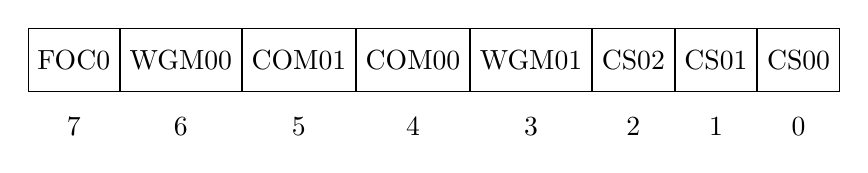
\begin{tikzpicture}[node distance=0cm]
    \node [draw, minimum width=1cm, minimum height=0.8cm] (foc) {FOC0};
    \node [draw, minimum width=1cm, minimum height=0.8cm, right=0cm of foc] (wgm0) {WGM00};
    \node [draw, minimum width=1cm, minimum height=0.8cm, right=0cm of wgm0] (com1) {COM01};
    \node [draw, minimum width=1cm, minimum height=0.8cm, right=0cm of com1] (com0) {COM00};
    \node [draw, minimum width=1cm, minimum height=0.8cm, right=0cm of com0] (wgm1) {WGM01};
    \node [draw, minimum width=1cm, minimum height=0.8cm, right=0cm of wgm1] (cs2) {CS02};
    \node [draw, minimum width=1cm, minimum height=0.8cm, right=0cm of cs2] (cs1) {CS01};
    \node [draw, minimum width=1cm, minimum height=0.8cm, right=0cm of cs1] (cs0) {CS00};
    
    \node [below=0.2cm of foc] {7};
    \node [below=0.2cm of wgm0] {6};
    \node [below=0.2cm of com1] {5};
    \node [below=0.2cm of com0] {4};
    \node [below=0.2cm of wgm1] {3};
    \node [below=0.2cm of cs2] {2};
    \node [below=0.2cm of cs1] {1};
    \node [below=0.2cm of cs0] {0};
\end{tikzpicture}
\end{center}

\begin{center}
\captionof{table}{TCCR0 Bits Function}
\begin{tabulary}{\linewidth}{|L|L|L|}
\hline
\textbf{Bit(s)} & \textbf{Name} & \textbf{Function} \\ \hline
7 & FOC0 & Force Output Compare \\ \hline
6,3 & WGM01:0 & Waveform Generation Mode \\ \hline
5,4 & COM01:0 & Compare Match Output Mode \\ \hline
2,1,0 & CS02:0 & Clock Select \\ \hline
\end{tabulary}
\end{center}

\begin{itemize}
    \item \keyword{WGM01:0}: Selects Normal, CTC, or PWM modes
    \item \keyword{COM01:0}: Defines OC0 pin behavior on compare match
    \item \keyword{CS02:0}: Sets clock source and prescaler (1, 8, 64, 256, 1024)
\end{itemize}
\end{solutionbox}

\begin{mnemonicbox}
\mnemonic{Forcing Waveforms, Comparing, Selecting Clock}
\end{mnemonicbox}

\questionmarks{3(a OR)}{3}{Explain AVR data memory.}

\begin{solutionbox}
AVR data memory consists of multiple sections for different types of data storage.

\textbf{Diagram:}

\begin{center}
\begin{tikzpicture}[node distance=1.2cm]
    % Top level - AVR Data Memory
    \node [draw, rectangle, minimum width=3cm, minimum height=0.8cm, rounded corners] (mem) {AVR Data Memory};
    
    % Hierarchical components below
    \node [draw, rectangle, minimum width=2.5cm, minimum height=0.7cm, below=of mem] (reg) {Registers};
    \node [draw, rectangle, minimum width=2.5cm, minimum height=0.7cm, below=of reg] (io) {I/O Registers};
    \node [draw, rectangle, minimum width=2.5cm, minimum height=0.7cm, below=of io] (sram) {Internal SRAM};
    \node [draw, rectangle, minimum width=2.5cm, minimum height=0.7cm, below=of sram] (eeprom) {EEPROM};
    
    % Connections from top to all components
    \draw [gtu arrow] (mem) -- (reg);
    \draw [gtu arrow] (mem) -- (io);
    \draw [gtu arrow] (mem) -- (sram);
    \draw [gtu arrow] (mem) -- (eeprom);
\end{tikzpicture}
\end{center}

\begin{itemize}
    \item \keyword{Registers}: 32 general-purpose registers (R0-R31)
    \item \keyword{I/O Memory}: Special function registers for peripherals
    \item \keyword{SRAM}: Internal RAM for variables (volatile)
    \item \keyword{EEPROM}: Non-volatile memory for persistent data
\end{itemize}
\end{solutionbox}

\begin{mnemonicbox}
\mnemonic{Registers I/O SRAM EEPROM}
\end{mnemonicbox}

\questionmarks{3(b OR)}{4}{Write an AVR C program to store 'G' into location 0x005F of EEPROM.}

\begin{solutionbox}
\begin{lstlisting}[language=C,caption={Write to EEPROM}]
#include <avr/io.h>
#include <avr/eeprom.h>

int main(void)
{
    // Store character 'G' to EEPROM location 0x005F
    eeprom_write_byte((uint8_t*)0x005F, 'G');
    
    while(1) {
        // Main loop
    }
    return 0;
}
\end{lstlisting}

\begin{itemize}
    \item \keyword{eeprom\_write\_byte()}: AVR library function to write to EEPROM
    \item \keyword{'G'}: ASCII value 71 (0x47) stored in EEPROM
    \item \keyword{0x005F}: Target EEPROM address
    \item \keyword{while(1)}: Infinite loop after writing
\end{itemize}
\end{solutionbox}

\begin{mnemonicbox}
\mnemonic{Write Once, Remember Forever}
\end{mnemonicbox}

\questionmarks{3(c OR)}{7}{Draw and explain TIFR register in detail.}

\begin{solutionbox}
Timer/Counter Interrupt Flag Register (TIFR) holds flags that indicate timer events.

\textbf{Diagram:}

\begin{center}
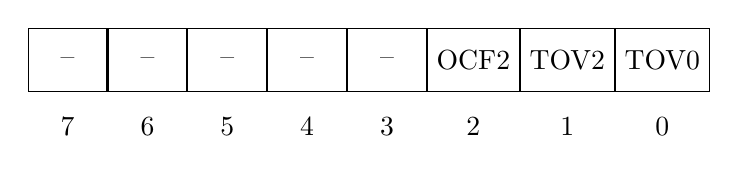
\begin{tikzpicture}[node distance=0cm]
    \node [draw, minimum width=1cm, minimum height=0.8cm] (b7) {--};
    \node [draw, minimum width=1cm, minimum height=0.8cm, right=0cm of b7] (b6) {--};
    \node [draw, minimum width=1cm, minimum height=0.8cm, right=0cm of b6] (b5) {--};
    \node [draw, minimum width=1cm, minimum height=0.8cm, right=0cm of b5] (b4) {--};
    \node [draw, minimum width=1cm, minimum height=0.8cm, right=0cm of b4] (b3) {--};
    \node [draw, minimum width=1cm, minimum height=0.8cm, right=0cm of b3] (ocf2) {OCF2};
    \node [draw, minimum width=1cm, minimum height=0.8cm, right=0cm of ocf2] (tov2) {TOV2};
    \node [draw, minimum width=1cm, minimum height=0.8cm, right=0cm of tov2] (tov0) {TOV0};
    
    \node [below=0.2cm of b7] {7};
    \node [below=0.2cm of b6] {6};
    \node [below=0.2cm of b5] {5};
    \node [below=0.2cm of b4] {4};
    \node [below=0.2cm of b3] {3};
    \node [below=0.2cm of ocf2] {2};
    \node [below=0.2cm of tov2] {1};
    \node [below=0.2cm of tov0] {0};
\end{tikzpicture}
\end{center}

\begin{center}
\captionof{table}{TIFR Bits Function}
\begin{tabulary}{\linewidth}{|L|L|L|}
\hline
\textbf{Bit} & \textbf{Name} & \textbf{Function} \\ \hline
0 & TOV0 & Timer/Counter0 Overflow Flag \\ \hline
1 & TOV2 & Timer/Counter2 Overflow Flag \\ \hline
2 & OCF2 & Output Compare Flag 2 \\ \hline
3-7 & -- & Reserved bits \\ \hline
\end{tabulary}
\end{center}

\begin{itemize}
    \item \keyword{TOV0}: Set when Timer0 overflows, cleared when ISR executes
    \item \keyword{TOV2}: Set when Timer2 overflows
    \item \keyword{OCF2}: Set when Timer2 compare match occurs
    \item \keyword{Flag Clearing}: Write `1' to bit to clear flag
\end{itemize}
\end{solutionbox}

\begin{mnemonicbox}
\mnemonic{Timers Overflow, Comparisons Flag}
\end{mnemonicbox}

\questionmarks{4(a)}{3}{Write different ways of generating delay in AVR.}

\begin{solutionbox}
AVR microcontrollers offer multiple methods to generate time delays.

\begin{center}
\captionof{table}{Delay Generation Methods}
\begin{tabulary}{\linewidth}{|L|L|L|}
\hline
\textbf{Method} & \textbf{Description} & \textbf{Precision} \\ \hline
Software Loops & CPU cycles counting & Low \\ \hline
Timer Interrupts & Hardware timers with ISR & High \\ \hline
Timer Polling & Hardware timers with flag checking & Medium \\ \hline
Delay Functions & Library functions (\_delay\_ms/\_delay\_us) & Medium \\ \hline
\end{tabulary}
\end{center}

\begin{itemize}
    \item \keyword{Software}: Simple but affected by optimizations
    \item \keyword{Hardware}: More accurate but requires timer setup
    \item \keyword{Library}: Convenient but limited to constant values
\end{itemize}
\end{solutionbox}

\begin{mnemonicbox}
\mnemonic{Loops, Interrupts, Polling, Functions}
\end{mnemonicbox}

\questionmarks{4(b)}{4}{Draw and explain interfacing of LM35 with ATmega32.}

\begin{solutionbox}
LM35 is a temperature sensor that outputs an analog voltage proportional to temperature.

\textbf{Circuit Diagram:}

\begin{center}
\begin{tikzpicture}[node distance=2cm]
    \node (vcc) {VCC (+5V)};
    \node [gtu block, below=1.5cm of vcc] (lm35) {LM35};
    \node [below=1.5cm of lm35] (gnd) {GND};
    \node [gtu block, right=3cm of lm35] (adc) {ATmega32\\ADC0 (PA0)};
    
    \path [draw] (vcc) -- (lm35);
    \path [gtu arrow] (lm35) -- node[above] {Analog Out} (adc);
    \path [draw] (lm35) -- (gnd);
\end{tikzpicture}
\end{center}

\begin{itemize}
    \item \keyword{Connection}: LM35 output to ADC0 (PA0) of ATmega32
    \item \keyword{Scaling}: 10mV/°C output (0°C = 0V, 25°C = 250mV)
    \item \keyword{ADC Setup}: Configure ADMUX to select ADC0
    \item \keyword{Calculation}: Temperature = (ADC\_value $\times$ 5 $\times$ 100) / 1024
\end{itemize}
\end{solutionbox}

\begin{mnemonicbox}
\mnemonic{Analog Voltage Converts Temperature}
\end{mnemonicbox}

\questionmarks{4(c)}{7}{Explain interfacing of MAX7221 with ATmega32 in detail.}

\begin{solutionbox}
MAX7221 is an LED display driver IC that connects to AVR using SPI communication.

\textbf{Circuit Diagram:}

\begin{center}
\begin{tikzpicture}[node distance=3cm]
    \node [draw, rectangle, minimum width=2.5cm, minimum height=2cm] (avr) {ATmega32};
    \node [draw, rectangle, minimum width=2.5cm, minimum height=2cm, right=of avr] (max) {MAX7221};
    \node [draw, rectangle, minimum width=2.5cm, minimum height=1.2cm, right=of max, align=center] (display) {7-Segment\\Display};
    
    % Three separate parallel signal connections with better spacing
    \draw [gtu arrow] ([yshift=7mm]avr.east) -- ([yshift=7mm]max.west) node[above, font=\tiny, pos=0.5] {PB7 (SCK)} node[below, font=\tiny, pos=0.5] {CLK};
    \draw [gtu arrow] (avr.east) -- (max.west) node[above, font=\tiny, pos=0.5] {PB5 (MOSI)} node[below, font=\tiny, pos=0.5] {DIN};
    \draw [gtu arrow] ([yshift=-7mm]avr.east) -- ([yshift=-7mm]max.west) node[above, font=\tiny, pos=0.5] {PB4 (SS)} node[below, font=\tiny, pos=0.5] {LOAD};
    
    % Connection to display
    \draw [gtu arrow] (max.east) -- (display.west);
\end{tikzpicture}
\end{center}

\begin{center}
\captionof{table}{Connections and Functionality}
\begin{tabulary}{\linewidth}{|L|L|L|}
\hline
\textbf{ATmega32 Pin} & \textbf{MAX7221 Pin} & \textbf{Function} \\ \hline
PB7 (SCK) & CLK & Serial Clock \\ \hline
PB5 (MOSI) & DIN & Data Input \\ \hline
PB4 (SS) & LOAD & Chip Select \\ \hline
\end{tabulary}
\end{center}

\begin{itemize}
    \item \keyword{SPI Mode}: Master mode, MSB first
    \item \keyword{Initialization}: Set decode mode, intensity, scan limit
    \item \keyword{Data Transfer}: Send address byte followed by data byte
    \item \keyword{Multiplexing}: Can drive up to 8 digits
    \item \keyword{Brightness Control}: 16 levels through intensity register
\end{itemize}
\end{solutionbox}

\begin{mnemonicbox}
\mnemonic{Send Clock Data Load Display}
\end{mnemonicbox}

\questionmarks{4(a OR)}{3}{Explain MAX232 line driver.}

\begin{solutionbox}
MAX232 is an IC that converts TTL/CMOS logic levels to RS-232 voltage levels for serial communication.

\textbf{Diagram:}

\begin{center}
\begin{tikzpicture}[node distance=3cm]
    \node [gtu block] (ttl) {TTL/CMOS\\(0/5V)};
    \node [gtu block, right=of ttl] (max232) {MAX232};
    \node [gtu block, right=of max232] (rs232) {RS-232\\($\pm$12V)};
    
    \node [above=0.5cm of max232] (c1) {C1+, C1-};
    \node [below=0.5cm of max232] (c2) {C2+, C2-};
    
    \path [gtu arrow, <->] (ttl) -- node[above, font=\small] {T1IN/R1OUT} (max232);
    \path [gtu arrow, <->] (max232) -- node[above, font=\small] {T1OUT/R1IN} (rs232);
\end{tikzpicture}
\end{center}

\begin{itemize}
    \item \keyword{Voltage Conversion}: TTL (0/5V) to RS-232 ($\pm$12V)
    \item \keyword{Charge Pumps}: Uses capacitors to generate required voltages
    \item \keyword{Applications}: Serial communication with PC, modems
    \item \keyword{Bidirectional}: Handles both transmit and receive signals
\end{itemize}
\end{solutionbox}

\begin{mnemonicbox}
\mnemonic{TTL To RS-232 Conversion}
\end{mnemonicbox}

\questionmarks{4(b OR)}{4}{Explain ADMUX register.}

\begin{solutionbox}
ADC Multiplexer Selection Register (ADMUX) controls analog input channel selection and result format.

\textbf{Diagram:}

\begin{center}
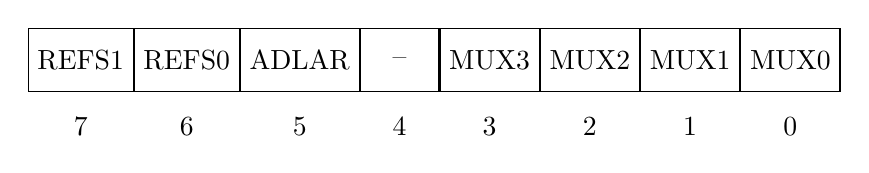
\begin{tikzpicture}[node distance=0cm]
    \node [draw, minimum width=1cm, minimum height=0.8cm] (refs1) {REFS1};
    \node [draw, minimum width=1cm, minimum height=0.8cm, right=0cm of refs1] (refs0) {REFS0};
    \node [draw, minimum width=1cm, minimum height=0.8cm, right=0cm of refs0] (adlar) {ADLAR};
    \node [draw, minimum width=1cm, minimum height=0.8cm, right=0cm of adlar] (b4) {--};
    \node [draw, minimum width=1cm, minimum height=0.8cm, right=0cm of b4] (mux3) {MUX3};
    \node [draw, minimum width=1cm, minimum height=0.8cm, right=0cm of mux3] (mux2) {MUX2};
    \node [draw, minimum width=1cm, minimum height=0.8cm, right=0cm of mux2] (mux1) {MUX1};
    \node [draw, minimum width=1cm, minimum height=0.8cm, right=0cm of mux1] (mux0) {MUX0};
    
    \node [below=0.2cm of refs1] {7};
    \node [below=0.2cm of refs0] {6};
    \node [below=0.2cm of adlar] {5};
    \node [below=0.2cm of b4] {4};
    \node [below=0.2cm of mux3] {3};
    \node [below=0.2cm of mux2] {2};
    \node [below=0.2cm of mux1] {1};
    \node [below=0.2cm of mux0] {0};
\end{tikzpicture}
\end{center}

\begin{center}
\captionof{table}{ADMUX Bit Functions}
\begin{tabulary}{\linewidth}{|L|L|L|}
\hline
\textbf{Bits} & \textbf{Name} & \textbf{Function} \\ \hline
7:6 & REFS1:0 & Reference Selection \\ \hline
5 & ADLAR & ADC Left Adjust Result \\ \hline
3:0 & MUX3:0 & Analog Channel Selection \\ \hline
\end{tabulary}
\end{center}

\begin{itemize}
    \item \keyword{REFS1:0}: Select voltage reference (AREF, AVCC, Internal)
    \item \keyword{ADLAR}: Result alignment in ADC registers
    \item \keyword{MUX3:0}: Select input channel (ADC0-ADC7)
\end{itemize}
\end{solutionbox}

\begin{mnemonicbox}
\mnemonic{Reference, Alignment, Multiplexer}
\end{mnemonicbox}

\questionmarks{4(c OR)}{7}{Discuss Two Wire serial Interface (TWI) in AVR.}

\begin{solutionbox}
Two Wire Interface (TWI) is AVR's implementation of I$^2$C protocol for communication with peripheral devices.

\textbf{Diagram:}

\begin{center}
\begin{tikzpicture}[node distance=2.5cm]
    \node [gtu block] (master) {Master AVR};
    \node [gtu block, right=of master] (slave1) {Slave 1};
    \node [gtu block, right=of slave1] (slave2) {Slave 2};
    
    \path [gtu arrow, <->] (master) -- node[above, font=\small] {SDA} (slave1);
    \path [gtu arrow, <->] (master.east) ++(0,-0.3) -- ++(2.5,0) node[below, font=\small, midway] {SCL};
    \path [gtu arrow, <->] (slave1) -- (slave2);
    \path [gtu arrow, <->] (slave1.east) ++(0,-0.3) -- ++(2.5,0);
\end{tikzpicture}
\end{center}

\begin{center}
\captionof{table}{TWI Characteristics}
\begin{tabulary}{\linewidth}{|L|L|}
\hline
\textbf{Feature} & \textbf{Description} \\ \hline
Pins & SCL (Serial Clock) and SDA (Serial Data) \\ \hline
Speed & Standard (100kHz), Fast (400kHz) \\ \hline
Addressing & 7-bit or 10-bit device addressing \\ \hline
Operation & Master or Slave mode \\ \hline
Bus Structure & Multi-master, multi-slave \\ \hline
\end{tabulary}
\end{center}

\begin{itemize}
    \item \keyword{Bidirectional}: Both devices can transmit and receive
    \item \keyword{Registers}: TWBR, TWCR, TWSR, TWDR, TWAR
    \item \keyword{ACK/NACK}: Acknowledgment for reliable transfers
    \item \keyword{Start/Stop}: Special conditions to begin/end transmission
    \item \keyword{Common Uses}: EEPROM, RTC, sensors, displays
\end{itemize}
\end{solutionbox}

\begin{mnemonicbox}
\mnemonic{Serial Clock And Data Transfers}
\end{mnemonicbox}

\questionmarks{5(a)}{3}{Draw circuit diagram to interface DC motor with ATmega32 using L293D motor driver.}

\begin{solutionbox}
L293D provides bidirectional drive current for controlling DC motors with microcontrollers.

\textbf{Circuit Diagram:}

\begin{center}
\begin{tikzpicture}[node distance=2.5cm]
    \node [gtu block] (avr) {ATmega32};
    \node [gtu block, right=of avr] (l293d) {L293D};
    \node [gtu block, right=of l293d] (motor) {DC Motor};
    \node [above=1cm of l293d] (vcc) {+5V Power};
    
    \path [gtu arrow] (avr) -- node[above, font=\small] {PD0} node[below, font=\small] {IN1} (l293d);
    \path [gtu arrow] (avr.east) ++(0,-0.3) -- ++(2.5,0) node[above, font=\small, midway] {PD1} node[below, font=\small, midway] {IN2};
    \path [gtu arrow] (l293d) -- node[above, font=\small] {OUT1, OUT2} (motor);
    \path [draw] (vcc) -- (l293d);
\end{tikzpicture}
\end{center}

\begin{itemize}
    \item \keyword{Control Pins}: PD0, PD1 control motor direction
    \item \keyword{Driver Power}: Separate for logic and motor
    \item \keyword{H-Bridge}: Enables forward/reverse operation
    \item \keyword{Enable Pin}: Can be used for PWM speed control
\end{itemize}
\end{solutionbox}

\begin{mnemonicbox}
\mnemonic{Direction Control Through Bridge}
\end{mnemonicbox}

\questionmarks{5(b)}{4}{Write features of on chip ADC in ATmega32.}

\begin{solutionbox}
ATmega32 features a versatile analog-to-digital converter for measuring analog signals.

\begin{center}
\captionof{table}{ATmega32 ADC Features}
\begin{tabulary}{\linewidth}{|L|L|}
\hline
\textbf{Feature} & \textbf{Specification} \\ \hline
Resolution & 10-bit \\ \hline
Channels & 8 single-ended inputs \\ \hline
Conversion Time & 65-260 $\mu$s \\ \hline
Reference Voltage & AREF, AVCC, or 2.56V internal \\ \hline
Accuracy & $\pm$2 LSB \\ \hline
Conversion Modes & Single and Free Running \\ \hline
Input Range & 0V to VREF \\ \hline
\end{tabulary}
\end{center}

\begin{itemize}
    \item \keyword{Successive Approximation}: Conversion technique
    \item \keyword{Multiplexer}: Selects among 8 input channels
    \item \keyword{Interrupt}: Optional interrupt on completion
    \item \keyword{Sampling Rate}: Up to 15 KSPS at maximum resolution
\end{itemize}
\end{solutionbox}

\begin{mnemonicbox}
\mnemonic{Multiple Channels, Ten-bit Resolution}
\end{mnemonicbox}

\questionmarks{5(c)}{7}{Explain Smart Irrigation System.}

\begin{solutionbox}
Smart Irrigation System automates watering based on environmental conditions using microcontroller technology.

\textbf{Diagram:}

\begin{center}
\begin{tikzpicture}[node distance=2cm, auto]
    \node [gtu block] (avr) {ATmega32};
    \node [gtu block, above left=1cm and 1cm of avr] (soil) {Soil Moisture\\Sensor};
    \node [gtu block, above=1cm of avr] (temp) {Temperature\\Sensor};
    \node [gtu block, above right=1cm and 1cm of avr] (hum) {Humidity\\Sensor};
    \node [gtu block, below left=1cm and 1cm of avr] (pump) {Water Pump\\Control};
    \node [gtu block, below=1cm of avr] (valve) {Valve\\Control};
    \node [gtu block, below right=1cm and 1cm of avr] (lcd) {LCD\\Display};
    \node [gtu block, left=2cm of avr] (rtc) {RTC Module};
    
    \path [gtu arrow] (soil) -- (avr);
    \path [gtu arrow] (temp) -- (avr);
    \path [gtu arrow] (hum) -- (avr);
    \path [gtu arrow] (avr) -- (pump);
    \path [gtu arrow] (avr) -- (valve);
    \path [gtu arrow] (avr) -- (lcd);
    \path [gtu arrow] (rtc) -- (avr);
\end{tikzpicture}
\end{center}

\begin{center}
\captionof{table}{System Components}
\begin{tabulary}{\linewidth}{|L|L|}
\hline
\textbf{Component} & \textbf{Function} \\ \hline
Soil Moisture Sensor & Measures water content in soil \\ \hline
Temperature/Humidity & Monitors environmental conditions \\ \hline
Water Pump & Delivers water when needed \\ \hline
Valves & Controls water flow to different zones \\ \hline
LCD Display & Shows system status \\ \hline
RTC Module & Tracks time for scheduled irrigation \\ \hline
\end{tabulary}
\end{center}

\begin{itemize}
    \item \keyword{Adaptive Control}: Adjusts watering based on conditions
    \item \keyword{Water Conservation}: Uses only necessary amount of water
    \item \keyword{Remote Monitoring}: Optional WiFi/GSM connectivity
    \item \keyword{Data Logging}: Records moisture levels and watering events
    \item \keyword{Battery Backup}: Ensures operation during power outages
\end{itemize}
\end{solutionbox}

\begin{mnemonicbox}
\mnemonic{Sense Moisture, Control Water Automatically}
\end{mnemonicbox}

\questionmarks{5(a OR)}{3}{Draw and explain pin diagram of L293D motor driver IC.}

\begin{solutionbox}
L293D is a quadruple half-H driver IC used for controlling motors and other inductive loads.

\textbf{Diagram:}

\begin{center}
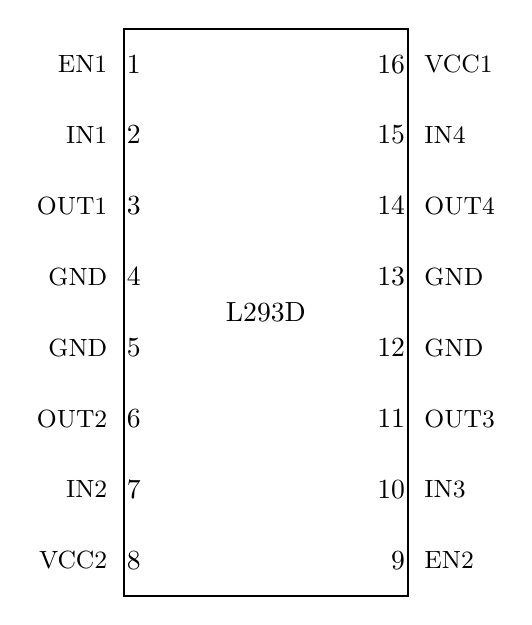
\begin{tikzpicture}[scale=0.9]
    % Draw the IC body
    \draw [thick] (0,0) rectangle (4,8);
    
    % Left side pins (1-8)
    \foreach \i/\label in {1/EN1, 2/IN1, 3/OUT1, 4/GND, 5/GND, 6/OUT2, 7/IN2, 8/VCC2} {
        \node [anchor=east, font=\small] at (-0.1, 8-\i*1+0.5) {\label};
        \node [anchor=west] at (-0.1, 8-\i*1+0.5) {\i};
    }
    
    % Right side pins (16-9)
    \foreach \i/\label in {16/VCC1, 15/IN4, 14/OUT4, 13/GND, 12/GND, 11/OUT3, 10/IN3, 9/EN2} {
        \pgfmathsetmacro{\pos}{8-(16-\i+1)*1+0.5}
        \node [anchor=west, font=\small] at (4.1, \pos) {\label};
        \node [anchor=east] at (4.1, \pos) {\i};
    }
    
    \node at (2,4) {L293D};
\end{tikzpicture}
\end{center}

\begin{itemize}
    \item \keyword{VCC1 (Pin 16)}: Logic supply voltage (5V)
    \item \keyword{VCC2 (Pin 8)}: Motor supply voltage (4.5V-36V)
    \item \keyword{EN1/EN2}: Enable inputs (can be PWM for speed control)
    \item \keyword{IN1-IN4}: Logic inputs to control direction
    \item \keyword{OUT1-OUT4}: Outputs to connect motors
    \item \keyword{GND}: Ground connections
\end{itemize}
\end{solutionbox}

\begin{mnemonicbox}
\mnemonic{Enable, Input, Output, Power}
\end{mnemonicbox}

\questionmarks{5(b OR)}{4}{List registers associated with ADC in AVR.}

\begin{solutionbox}
AVR's ADC system uses several registers to control its operation and store results.

\begin{center}
\captionof{table}{ADC Registers}
\begin{tabulary}{\linewidth}{|L|L|L|}
\hline
\textbf{Register} & \textbf{Function} & \textbf{Description} \\ \hline
ADMUX & Multiplexer & Channel selection and reference options \\ \hline
ADCSRA & Control \& Status & Control bits and flags \\ \hline
ADCH & Data High & High byte of conversion result \\ \hline
ADCL & Data Low & Low byte of conversion result \\ \hline
SFIOR & Special Function & ADC trigger source selection \\ \hline
\end{tabulary}
\end{center}

\begin{itemize}
    \item \keyword{ADMUX}: Channel and reference selection
    \item \keyword{ADCSRA}: Enable ADC, start conversion, prescaler
    \item \keyword{ADCH/ADCL}: Result registers (10-bit value)
    \item \keyword{SFIOR}: Auto-trigger sources (Timer, External)
\end{itemize}
\end{solutionbox}

\begin{mnemonicbox}
\mnemonic{Multiplexer Controls And Delivers Results}
\end{mnemonicbox}

\questionmarks{5(c OR)}{7}{Explain IoT based home automation system.}

\begin{solutionbox}
IoT home automation connects household devices to the internet for remote monitoring and control.

\textbf{Diagram:}

\begin{center}
\begin{tikzpicture}[node distance=2cm, auto]
    \node [gtu block] (internet) {Internet};
    \node [gtu block, below=1cm of internet] (gateway) {WiFi Gateway};
    \node [gtu block, below=1cm of gateway] (avr) {AVR Controller};
    
    \node [gtu block, below left=1cm and 0.5cm of avr] (light) {Light Control};
    \node [gtu block, below=1cm of avr] (fan) {Fan Control};
    \node [gtu block, below right=1cm and 0.5cm of avr] (door) {Door Lock};
    
    \node [gtu block, right=2cm of avr] (temp) {Temperature\\Sensors};
    \node [gtu block, below=0.5cm of temp] (motion) {Motion\\Sensors};
    
    \node [gtu block, left=2cm of gateway] (app) {Mobile App};
    \node [gtu block, right=2cm of gateway] (cloud) {Cloud Services};
    
    \path [gtu arrow, <->] (internet) -- (gateway);
    \path [gtu arrow, <->] (gateway) -- (avr);
    \path [gtu arrow] (avr) -- (light);
    \path [gtu arrow] (avr) -- (fan);
    \path [gtu arrow] (avr) -- (door);
    \path [gtu arrow] (temp) -- (avr);
    \path [gtu arrow] (motion) -- (avr);
    \path [gtu arrow, <->] (gateway) -- (app);
    \path [gtu arrow, <->] (gateway) -- (cloud);
\end{tikzpicture}
\end{center}

\begin{center}
\captionof{table}{System Components}
\begin{tabulary}{\linewidth}{|L|L|}
\hline
\textbf{Component} & \textbf{Function} \\ \hline
Controller & Processes sensor data and commands \\ \hline
Sensors & Monitor environmental conditions \\ \hline
Actuators & Control appliances and systems \\ \hline
Communication & WiFi/Ethernet/Bluetooth connectivity \\ \hline
Gateway & Connects local network to internet \\ \hline
Mobile App & User interface for remote control \\ \hline
\end{tabulary}
\end{center}

\begin{itemize}
    \item \keyword{Remote Access}: Control home from anywhere
    \item \keyword{Scheduling}: Automate device operation based on time
    \item \keyword{Voice Control}: Integration with digital assistants
    \item \keyword{Energy Monitoring}: Track power consumption
    \item \keyword{Security}: Alerts for unusual activities
    \item \keyword{Scene Setting}: One-touch control of multiple devices
\end{itemize}
\end{solutionbox}

\begin{mnemonicbox}
\mnemonic{Connect, Control, Automate, Monitor}
\end{mnemonicbox}

\end{document}
